Synonims: system, application, service

Definitions:
\begin{itemize}
    \item Performance: With the term \textbf{permormance} we refer to the distinction of the farmer's productivity such as they produce the crops well or not. It will be categorized by 3 different types (high performer, medium performer, low performer).
    \item Incentive status (none): With the term \textbf{incentive status (none)} we refer to the condition that the incentive has not prepared yet.
    \item Incentive status (prepared): With the term \textbf{incentive status (prepared)} we refer to the condition that the incentive exist at a warehouse, but it hasn't been sent yet.
    \item Incentive status (sent): With the term \textbf{incentive status (sent)} we refer to the condition that the incentive has been sent to the farmer, but the comfirmation from farmer does't exist.
    \item Incentive status (received): With the term \textbf{incentive status (received)} we refer to the condition that the farmer comfirmed that they have received the incentive successfully.

\end{itemize}

\begin{table}[H]
    \centering
    \begin{tabular}{|l|p{0.75\textwidth}|}
        \hline % ---------------------------------------------------------------------
    	\textsc{id}                 &   1\\
    	\hline % ---------------------------------------------------------------------
    	\textsc{Name}               &   Visualize the performance data of each farmer\\
    	\hline % ---------------------------------------------------------------------
    	\textsc{Actors}             &   Policy maker\\
    	\hline % ---------------------------------------------------------------------
    	\textsc{Entry conditions}   &   Policy maker has logged in\\
    	\hline % ---------------------------------------------------------------------
    	\textsc{Event flow}         &   \footnotesize
            	                        \begin{itemize}
                                    	    \item Policy maker presses the button “Farmer’s performance”
                                    		\item The system displays a page with list of farmer divided by performances
                                    		\item Policy maker selects interested farmer’s name
                                    		\item The system shows the detailed information about farmer’s production
                                        \end{itemize}\\
        \hline % ---------------------------------------------------------------------
        \textsc{Exit conditions}    &  The system returns to the main page of policy maker\\
    	\hline % ---------------------------------------------------------------------
    	\textsc{Output}             &  \begin{itemize}
    	    \item Policy maker has obtained the data they were looking for
    	\end{itemize}\\
    	\hline % ---------------------------------------------------------------------
    	\textsc{Exceptions}         &  Policy maker couldn’t find the name of farmer who should exist\\
    	\hline % ---------------------------------------------------------------------
        
    \end{tabular}
    \caption{\label{tab:visualize_farmer_performance}Use case table that describes one of the policy maker functional requirements:  the capability of visualizing the farmer's information categorized by their performance} %TODO: add caption
\end{table}

\begin{figure}[H]
    \centering
    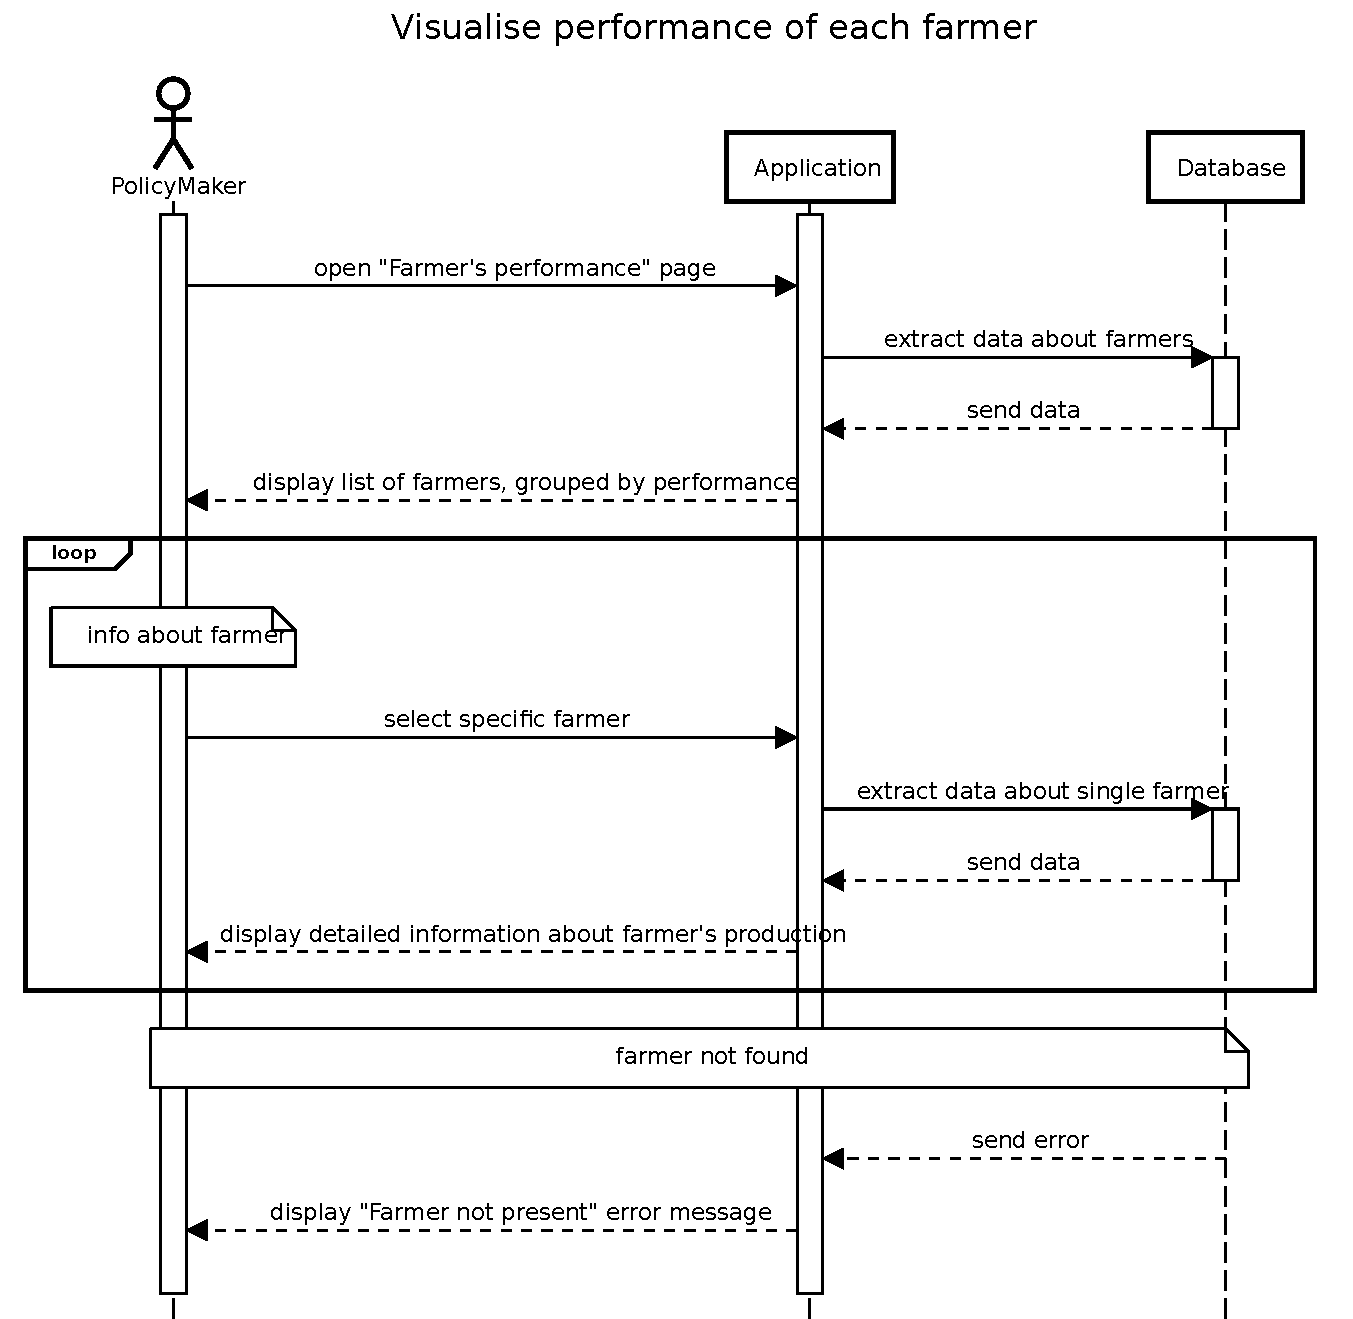
\includegraphics[scale=0.5]{Images/Sequence diagrams/PolicyMaker - visualize performance.pdf}
    \caption{Caption}
    \label{fig:my_label}
\end{figure}

\begin{table}[H]
    \centering
    \begin{tabular}{|l|p{0.75\textwidth}|}
        \hline % ---------------------------------------------------------------------
    	\textsc{id}                 &   2\\
    	\hline % ---------------------------------------------------------------------
    	\textsc{Name}               &   Visualize the incentive status data\\
    	\hline % ---------------------------------------------------------------------
    	\textsc{Actors}             &   Policy maker\\
    	\hline % ---------------------------------------------------------------------
    	\textsc{Entry conditions}   &   Policy maker has logged in\\
    	\hline % ---------------------------------------------------------------------
    	\textsc{Event flow}         &   \footnotesize
            	                        \begin{itemize}
                                    	    \item Policy maker presses the button “Farmer’s performance”
                                    		\item The system displays a page with list of farmer divided by performance, at the place of high performer there will be a column which clarifies the status of incentive 
                                       		\item Policy maker selects interested farmer’s incentive column
                                    		\item The system shows the detailed information about farmer’s incentive status
                                        \end{itemize}\\
        \hline % ---------------------------------------------------------------------
        \textsc{Exit conditions}    &  The system returns to the main page of policy maker\\
    	\hline % ---------------------------------------------------------------------
    	\textsc{Output}             &  \begin{itemize}
    	    \item Policy maker has obtained the data they were looking for
    	\end{itemize}\\
    	\hline % ---------------------------------------------------------------------
    	\textsc{Exceptions}         &  Policy maker couldn’t find the name of farmer who should exist\\
    	\hline % ---------------------------------------------------------------------
        
    \end{tabular}
    \caption{\label{tab:visualize_incentives}Use case table that describes one of the policy maker functional requirements:  the capability of tracking the incentive statuses} %TODO: add caption
\end{table}

\begin{figure}[H]
    \centering
    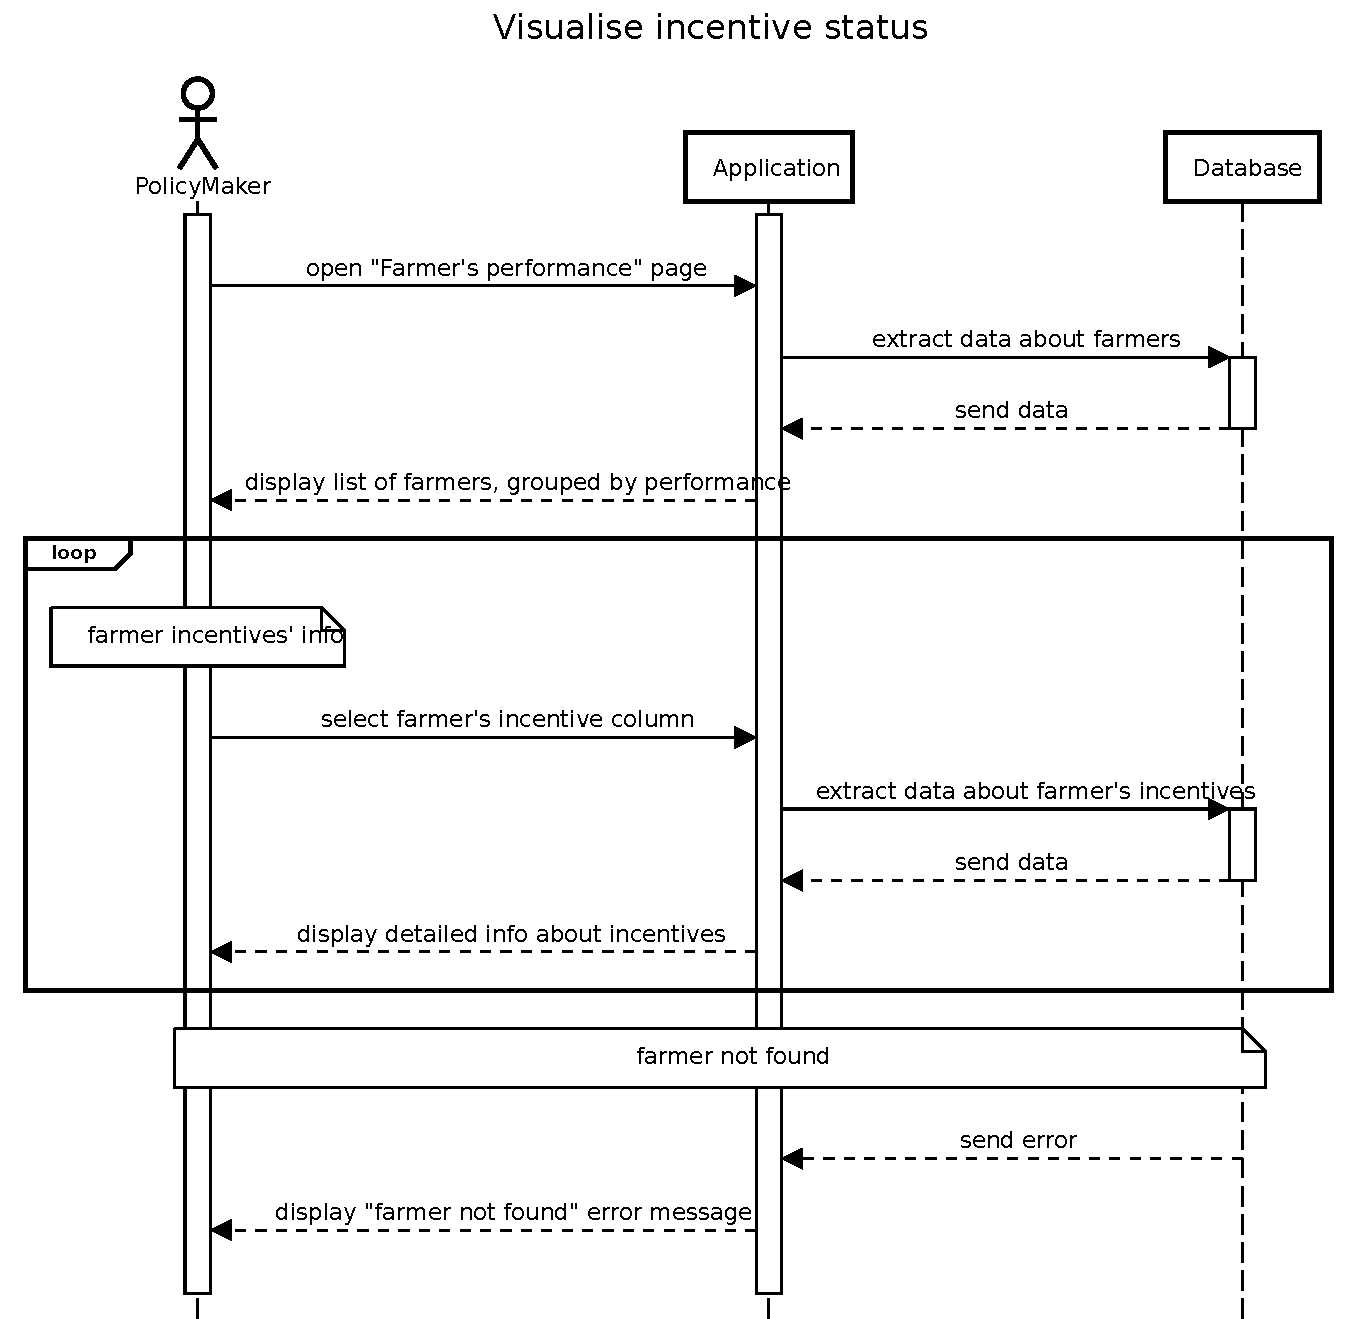
\includegraphics[scale=0.5]{Images/Sequence diagrams/PolicyMaker - visualise incentive status.pdf}
    \caption{Caption}
    \label{fig:my_label}
\end{figure}

\begin{table}[H]
    \centering
    \begin{tabular}{|l|p{0.75\textwidth}|}
        \hline % ---------------------------------------------------------------------
    	\textsc{id}                 &   3\\
    	\hline % ---------------------------------------------------------------------
    	\textsc{Name}               &   Visualize the correlation of history of visiting and improvement of farmer's performance\\
    	\hline % ---------------------------------------------------------------------
    	\textsc{Actors}             &   Policy maker\\
    	\hline % ---------------------------------------------------------------------
    	\textsc{Entry conditions}   &   Policy maker has logged in\\
    	\hline % ---------------------------------------------------------------------
    	\textsc{Event flow}         &   \footnotesize
            	                        \begin{itemize}
                                    	    \item Policy maker presses the button “Performance transition”
                                    		\item The system displays a page with categorized farmer, also it highlights the farmers who have improved their performance significantly within a year
                                    		\item Policy maker selects interested farmer’s name
                                    		\item The system shows the detailed information about farmer’s monthly performance transition 
                                        \end{itemize}\\
        \hline % ---------------------------------------------------------------------
        \textsc{Exit conditions}    &  The system returns to the main page of policy maker\\
    	\hline % ---------------------------------------------------------------------
    	\textsc{Output}             &  \begin{itemize}
    	    \item Policy maker has obtained the data they were looking for
    	\end{itemize}\\
    	\hline % ---------------------------------------------------------------------
    	\textsc{Exceptions}         &  Policy maker couldn’t find the name of farmer who should exist\\
    	\hline % ---------------------------------------------------------------------
        
    \end{tabular}
    \caption{\label{tab:visualize_iprovement}Use case table that describes one of the policy maker functional requirements:  the capability of tracking the transition of farmer's performance due to the visits of agronomists} %TODO: add caption
\end{table}

\begin{figure}[H]
    \centering
    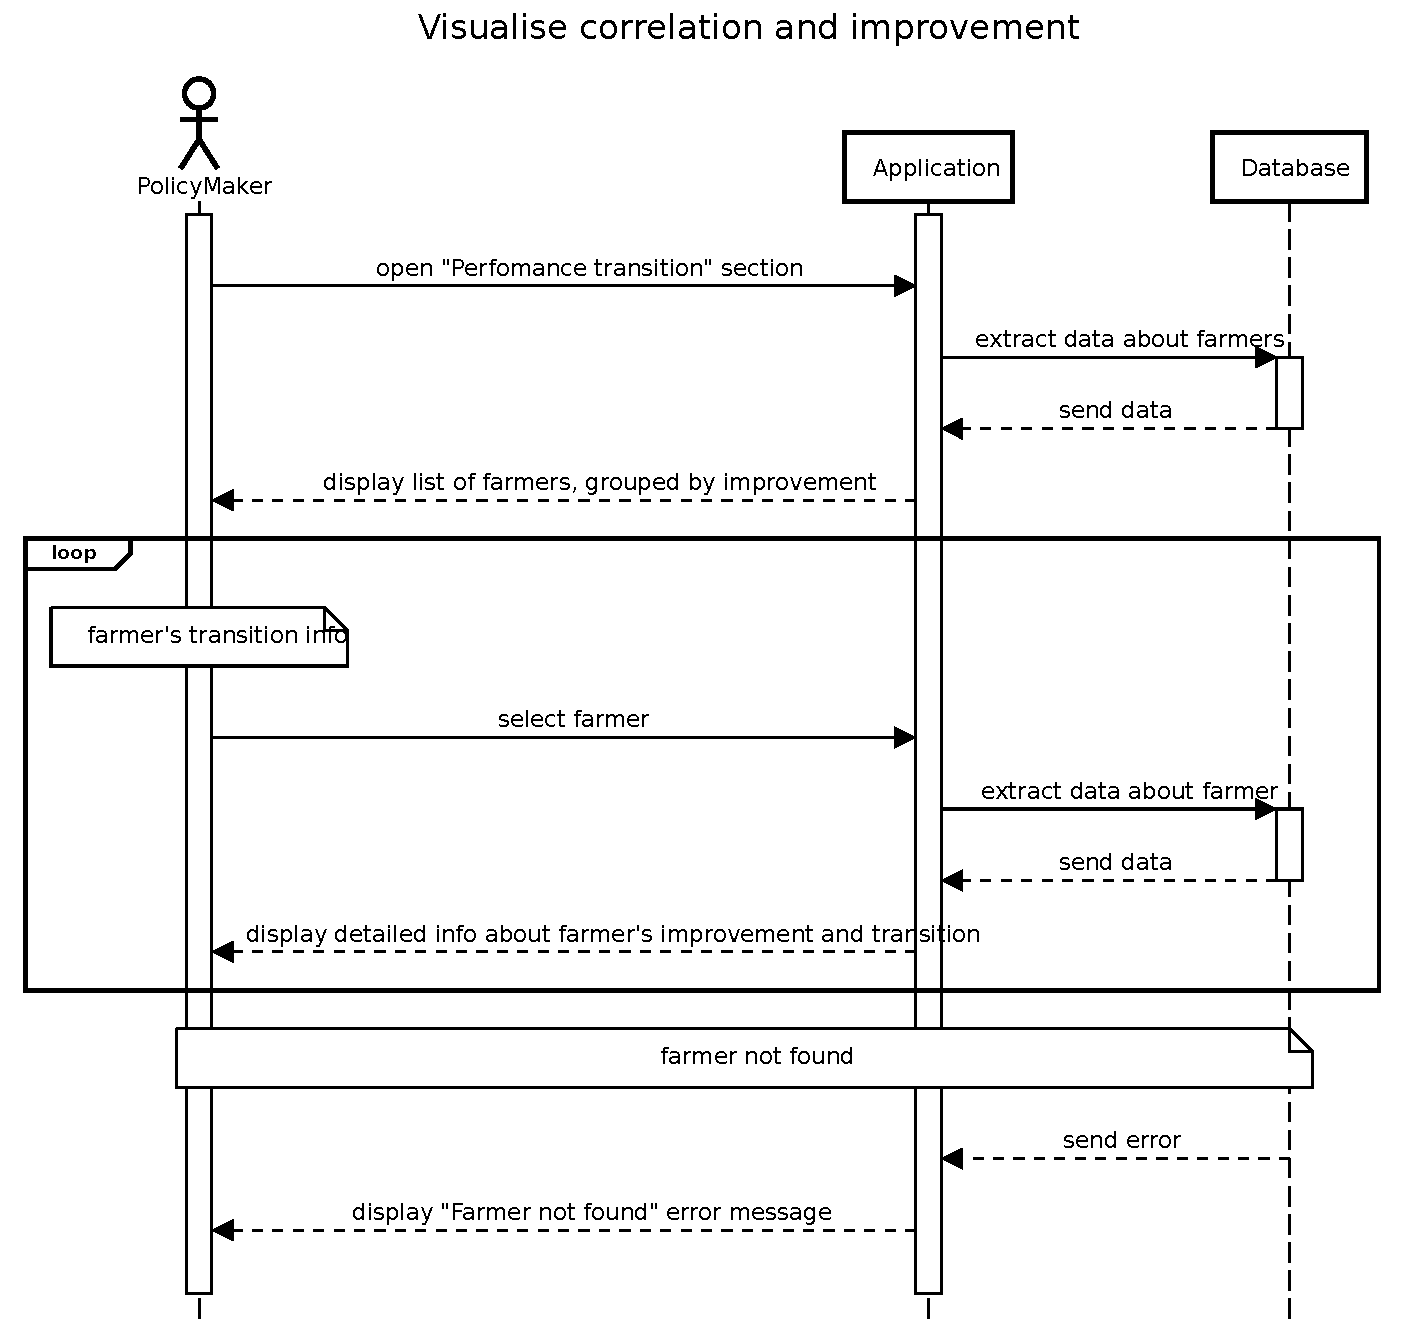
\includegraphics[scale=0.5]{Images/Sequence diagrams/PolicyMaker - visualise correlation and improvement.pdf}
    \caption{Caption}
    \label{fig:my_label}
\end{figure}